Die Projektplanung ist der wichtigsten Teil des Projektmanagements. Die
Rahmenbedingungen für das Projekt wurden bereits beim Antrag der Diplomarbeit
festgelegt.

\subsection{OpenProject}
Für das Projektmanagement wird die Softwareanwendung
OpenProject\footnote{https://www.openproject.org} verwendet. Der Vorteil dieser
Software ist, dass diese nicht wie eine normale Desktop-Anwendung lokal auf dem
Rechner des Benutzers läuft, sondern auf einem Server. Der Vorteil davon ist,
dass das kollaborative arbeiten stark vereinfacht wird. OpenProject biete die
Möglichkeit die Anwendung in der eigenen Infrastruktur zu installieren und
bietet somit eine vollständige Kontrolle über die eigenen Daten.

\subsection{Phasen}
Die gesamte Projektplanung ist in vier Phasen aufgeteilt:

\begin{itemize}
  \item \textbf{Themenfindungsphase}\\
  In der Themenfindungsphase geht es um das finden des expliziten Themas, dabei
  werden die Rahmenbedingungen mit dem Betreuer festgelegt.
  \item \textbf{Planungsphase}\\
  In der Planungsphase werden Arbeitspakete erstellt und den einzelnen
  Mitgliedern des Projektes verteilt.
  \item \textbf{Entwicklungsphase}
  Die Entwicklungsphase ist der längste und wichtigste Teil des Projekts, dabei
  werden alle Arbeitspakete so gut wie möglich abgearbeitet.
  \item \textbf{Abschlussphase}
  In der Abschlussphase geht es um das Schreiben der Diplomarbeit so wie letzte
  technische Feinschliffe in der Software und Hardware.
\end{itemize}
\subsection{Arbeitspakete}
Grundsätzlich sind die Arbeitspakte in drei Themenbereiche aufgeteilt:

\begin{itemize}
  \item Kennzeichenerkennung (Samuel)
  \item Fahrzeugerkennung (Dennis)
  \item Webinterface (Philipp)
\end{itemize}

\begin{figure}[H]
  \centering
  \frame{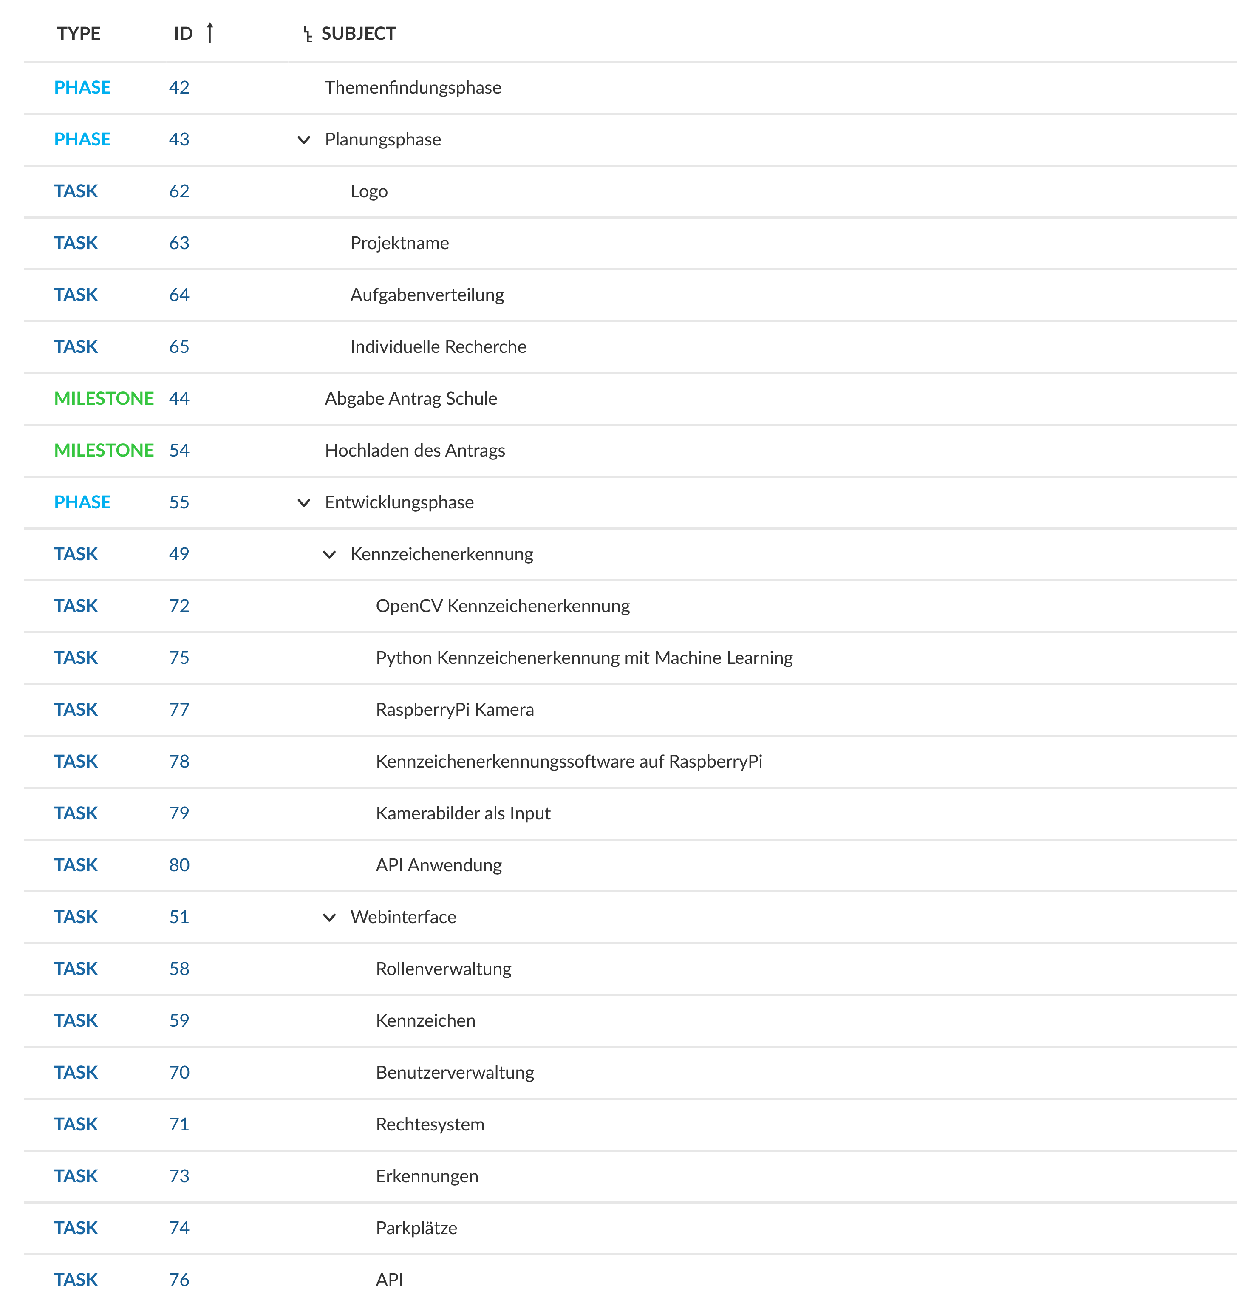
\includegraphics[width=1\linewidth]{arbeitspakete_1.pdf}}
  \caption{Arbeitspakete Teil 1}
\end{figure}

\begin{figure}[H]
  \centering
  \frame{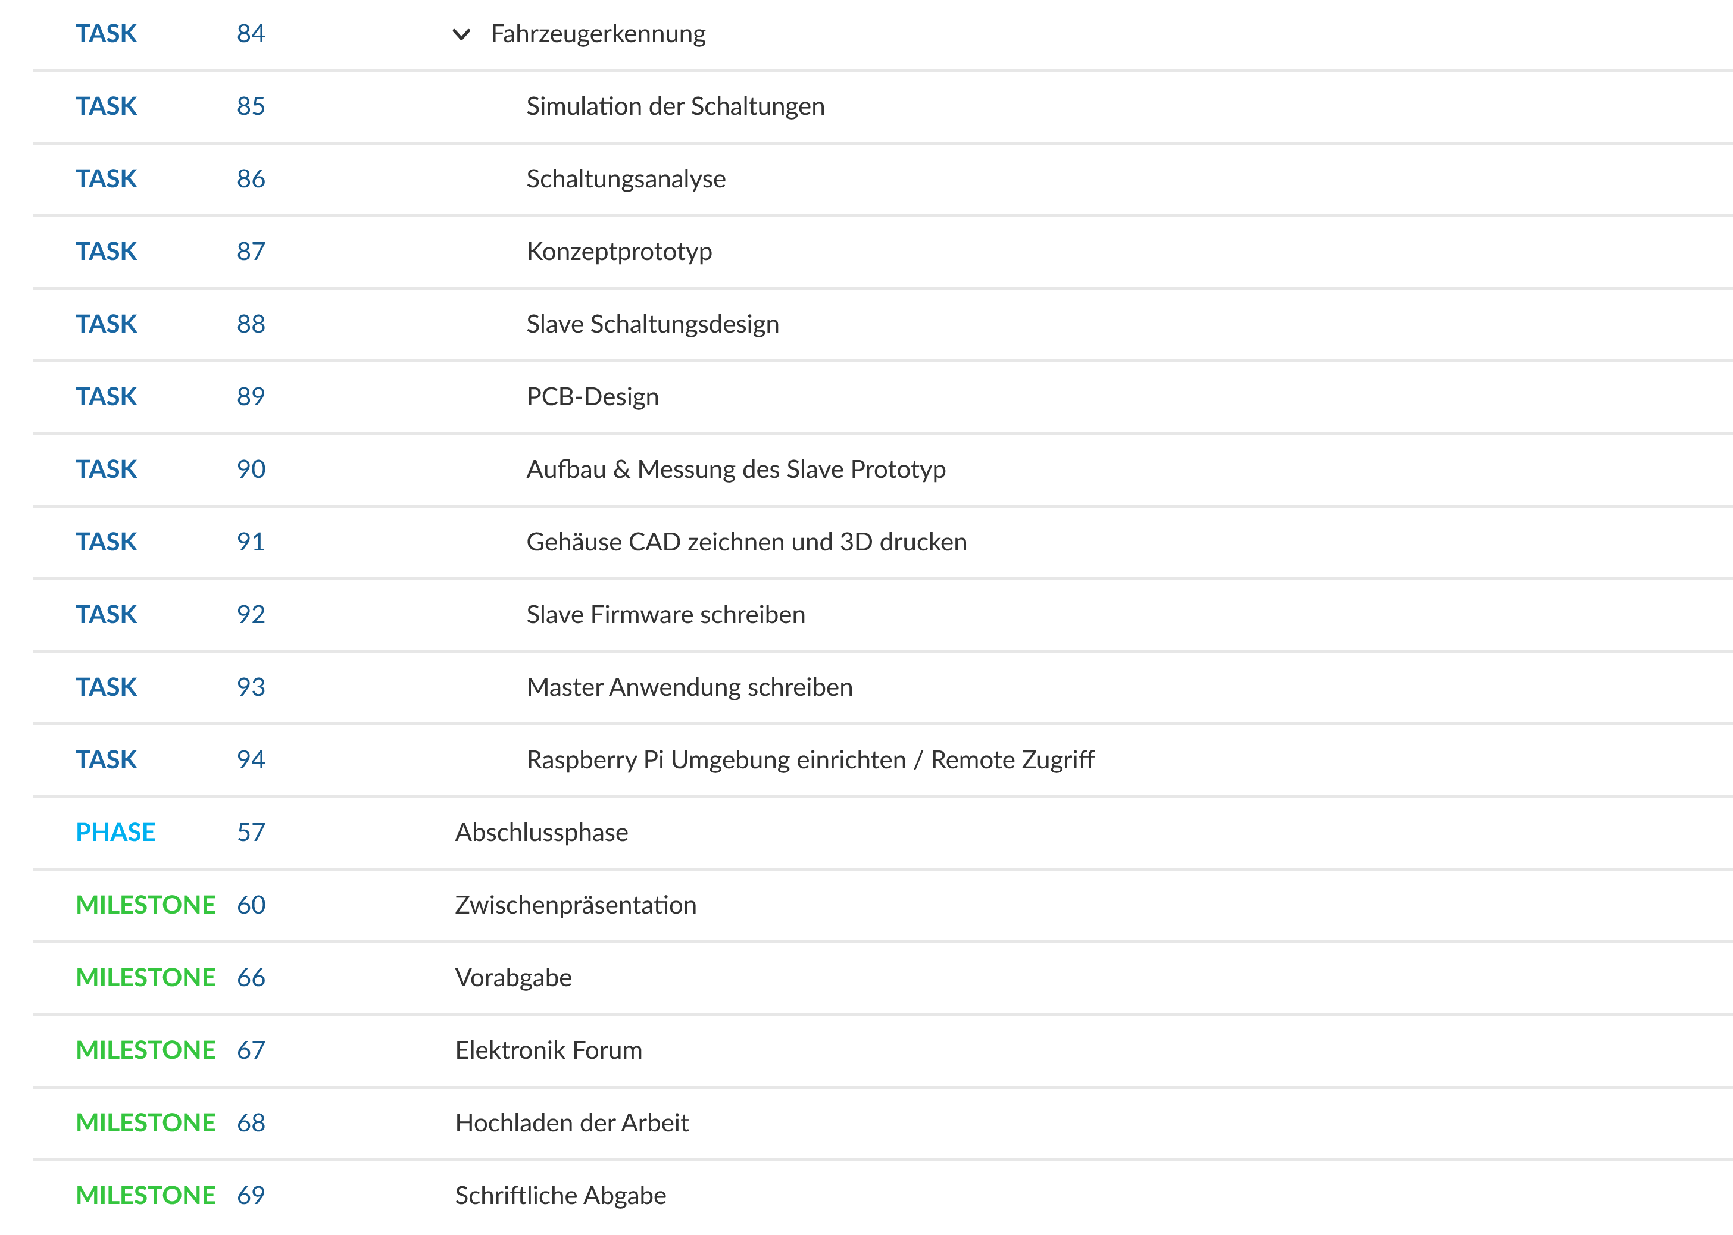
\includegraphics[width=1\linewidth]{arbeitspakete_2.pdf}}
  \caption{Arbeitspakete Teil 2}
\end{figure}

\subsection{Gantt-Diagramm}
Gantt-Diagramme oder Balkenplan sind spezielle Balkendiagramme um verschiedene
Arbeitspakete oder Aktivitäten auf einer Zeitachse auf einer Zeitachse
darzustellen.

\begin{figure}[H]
  \centering
  \frame{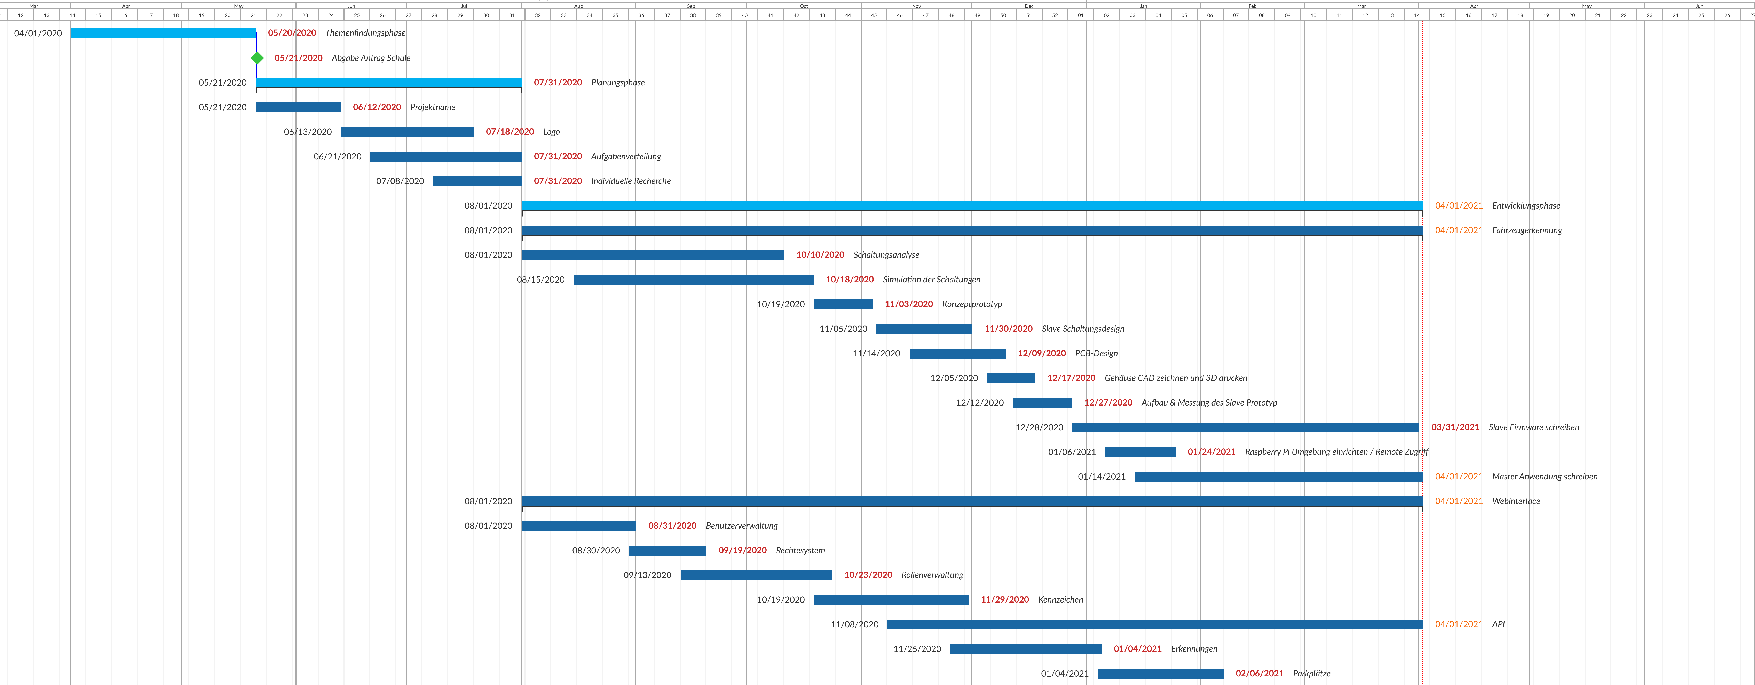
\includegraphics[width=1\linewidth]{gantt_1.pdf}}
  \caption{Gantt-Chart Teil 1}
\end{figure}

\begin{figure}[H]
  \centering
  \frame{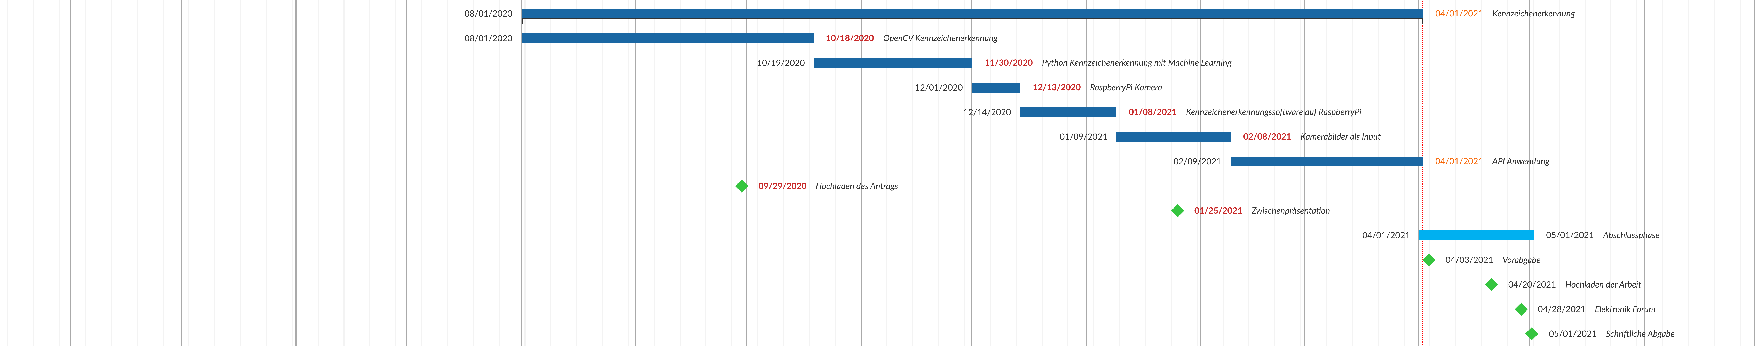
\includegraphics[width=1\linewidth]{gantt_2.pdf}}
  \caption{Gantt-Chart Teil 2}
\end{figure}

\subsection{Zeitaufwendungen}

Die Dokumentation der Zeitaufwendungen erfolgt über ein
Tabellenkalkulationsprogramm, dabei wird folgendes Dokumentiert:

\begin{itemize}
  \item Datum
  \item Typ
  \item Beschreibung
  \item Aufwand in Stunden
\end{itemize}

Die komplette Übersicht der aufgewendeten Stunden ist im Anhang ersichtlich.

\begin{table}[H]
  \centering
  \begin{tabular}{@{}ll@{}}
  \toprule
  \multicolumn{2}{c}{\textbf{Zeitaufwendungen}} \\ \midrule
  Philipp Kraft             & 181.5 h           \\
  Dennis Köb                & 177 h             \\
  Samuel Bleiner            & 112.5 h           \\ \midrule
  Gesamtaufwand:            & 471 h             \\ \bottomrule
  \end{tabular}
  \caption{Zeitaufwendungen Übersicht}
\end{table}